% DEFINED:   sec:rnn-alice, fig:ch05-rnn-loss
% RESOLVED:  ch:fixed-context-lm (backward into Part II)
% FORWARD:   (none; the Transformer is prose-only in a later section)

\section{The experiment: char-level Alice, and the comparison with
  Bengio}\label{sec:rnn-alice}

We train a vanilla \texttt{RNNCell} and a \texttt{Linear} output projection
on the first $30{,}000$ characters of \emph{Alice's Adventures in
Wonderland}, the same corpus and the same $75$-character vocabulary
\Cref{ch:fixed-context-lm} used. That is the point of reusing it: the
recurrent network and the fixed-context model are trained on identical data,
so the comparison at the end is fair. The model reads one character at a
time, and its job at each step is to predict the next character from the
state that summarizes everything read so far.

The configuration is small on purpose. The cell is
\texttt{RNNCell(input\_size=75, hidden\_size=64)}, the head is
\texttt{Linear(64, 75)}, and the loss is \texttt{SoftmaxCrossEntropy}.
Sequences are unrolled $32$ steps for backpropagation through time, the
learning rate is $0.5$ against the mean per-timestep gradient, the global
gradient norm is clipped to $5$, and training runs $15$ epochs over the
$937$ non-overlapping chunks the corpus cuts into. The parameter count is
the input-to-hidden matrix, the recurrent matrix, the hidden bias, and the
output projection with its bias:
\[
  64 \cdot 75 + 64 \cdot 64 + 64 + 75 \cdot 64 + 75 = 13{,}835.
\]

A model that guesses the next character uniformly at random scores
$\log 75 \approx 4.32$ nats per character, the entropy of the uniform
distribution over the vocabulary. That is the baseline to beat. Over the
$15$ epochs the mean per-character loss descends steadily,
\[
  4.32 \;\to\; 3.09 \;\to\; 2.40 \;\to\; 2.17 \;\to\; \cdots \;\to\; 2.05
\]
nats per character (the values shown are the start, then epochs one, five,
and ten, then the end), finishing at $2.05$ nats per character, a perplexity
of $e^{2.05} \approx 7.79$. \Cref{fig:ch05-rnn-loss} plots the full
trajectory. The descent is smooth and still gently sloping at epoch $15$:
unlike the fixed-context model, which did most of its work in the first
epoch, the recurrent network improves gradually across all $15$, because
each chunk is one sequential SGD step rather than thousands of independent
window updates.

\begin{figure}[ht]
  \centering
  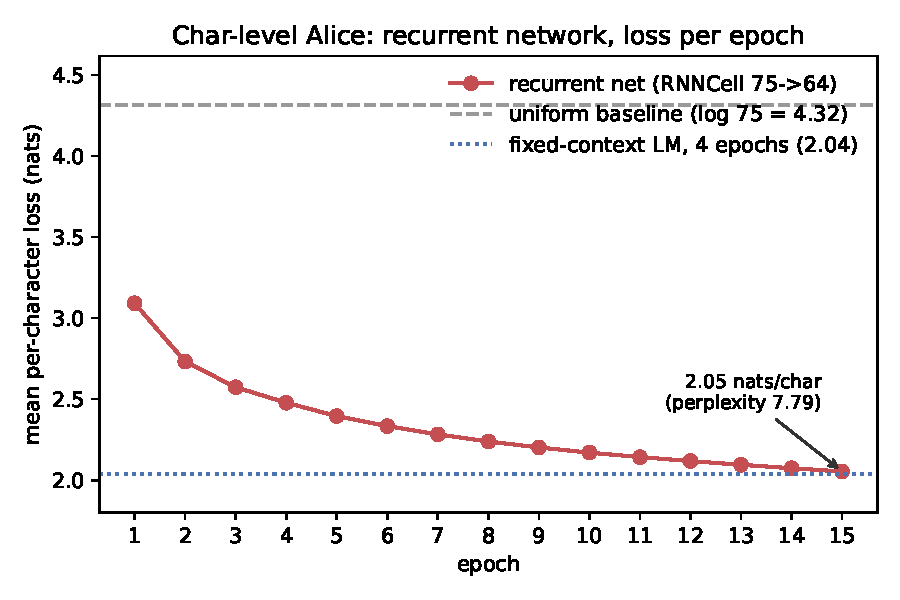
\includegraphics[width=0.7\linewidth]{figures/ch05-rnn-loss.pdf}
  \caption{Char-level Alice: mean per-character loss per epoch for the
    recurrent network (\texttt{RNNCell} $75 \to 64$, then
    \texttt{Linear} $64 \to 75$), trained by backpropagation through time
    with sequence length $32$ and gradient clipping. The dashed line is the
    uniform-random baseline, $\log 75 \approx 4.32$ nats per character. The
    dotted line marks the fixed-context language model of
    \Cref{ch:fixed-context-lm}, which reached $2.04$ nats per character in
    four epochs on the same corpus. Over $15$ epochs the recurrent network
    descends to $2.05$ nats per character (perplexity $7.79$), a comparable
    endpoint reached by a different route.}
  \label{fig:ch05-rnn-loss}
\end{figure}

\textbf{What the samples look like.} The clearest view of what the model
learns is to generate from it. At each epoch boundary we seed the state with
\texttt{"Alice "} and roll forward $200$ characters at temperature $0.8$ (the
paired notebook stores the full samples; short excerpts are quoted here).
After one epoch, at loss $3.09$, the output is close to random characters
with spaces at roughly plausible intervals:
\begin{quote}
\ttfamily Alice wh tsbi ta teca aa mu rea meam ifs n r ne san uou d hl au t
iiee thgo to aaf moghe ior te the \ldots
\end{quote}
By the fifth epoch, at loss $2.40$, the character distribution is right and
word-like fragments appear, with common short words surfacing intact:
\begin{quote}
\ttfamily Alice Aa's verind thing to Hop, ang ``a thand pad wed nof the hact
touro the varnt wand wave \ldots
\end{quote}
By the fifteenth epoch, at loss $2.05$, the fragments are English-shaped,
with many real words and the beginnings of local phrasing:
\begin{quote}
\ttfamily Alice out it, and the little wind she Mace sait a dit \ldots and
hall thest wore that hereed and \ldots she madeand theme was dow \ldots
\end{quote}
The trajectory is the classic char-level recurrent arc: random-character
noise, then the character distribution as vowels and consonants alternate
and spacing lands, then word-like fragments and recognizable short words,
then sentences that look locally English but drift in meaning across longer
spans. That drift is the vanishing-gradient limit showing in the output. The
state holds enough to get spelling and short words right, and not enough to
keep a thought coherent across a clause. A larger hidden state, longer
unrolls, and gated cells would push the coherence further; the vanilla cell
at modest scale and pure-Python compute lands here. The arc is the lesson,
and the absolute quality is the next chapter's concern.

\subsection*{The comparison with Bengio}

This is where the two architectures meet on the same data. The
fixed-context model of \Cref{ch:fixed-context-lm} reached $2.04$ nats per
character in about four epochs over $29{,}992$ independent eight-character
windows. The recurrent network reaches $2.05$ nats per character over
$15$ epochs of backpropagation through time. The endpoints are essentially
the same. The routes are not, and the difference is the whole point of
setting them side by side.

Start with what each one gives up. The fixed-context model gives up any
reach past its window. It conditions on exactly the last $N$ tokens and
forgets everything older by construction, so a dependency that spans more
than $N$ characters is simply invisible to it. The recurrent network gives
up nothing of the kind in principle: the state is a running summary of the
entire past, so there is no hard wall at $N$. What it gives up instead is
reliable access to the distant past in practice. The
vanishing-gradient problem means the gradient that would teach it to use a
far-back input decays before it arrives, so the effective memory is a few
dozen steps, not the whole sequence. One model has a sharp, known horizon;
the other has a soft, unreliable one.

Now what each one gains. The fixed-context model gains training simplicity,
and it is hard to overstate how much. Every window-target pair is
independent, so training is ordinary mini-batch classification with no
ordering to respect, no state to thread, and no unrolling. There is no long
product of Jacobians, so the gradient is well-behaved and the model converges
in a handful of epochs. The recurrent network gains the unbounded-in-principle
memory and the parameter economy that comes with it: one shared recurrent
matrix carries the past, rather than a separate slab of head weights per
window position, which is why it reaches a comparable loss with $13{,}835$
parameters against the fixed-context model's $14{,}331$. It pays for that
reach with sequential training, a fragile gradient, and the four-times-longer
schedule the trajectory shows.

For char-level Alice the contest is close to a draw, and that is itself
informative. Character prediction leans heavily on local structure,
morphology, word boundaries, common bigrams and trigrams, all of which live
well inside an eight-character window, so the fixed-context model's hard
horizon rarely bites and its training simplicity wins it a fast,
comparable result. The recurrent network's extra reach buys little here
because there is little long-range structure to reach for at the character
level. The recurrent prior earns its premium only when the data carries
dependencies longer than any fixed window one would be willing to pay for,
and even then only to the extent the vanishing gradient lets the state
actually carry them. That last qualification is exactly the gap the next
chapter sets out to close.
